% Fundamentação teórica
\section{Fundamenta\ca o Te\oh rica}

\label{pro:fundamentacao}

Linguagem de Programa\ca o \eh\ a nota\ca o utilizada para descrever computa\co es, comumente chamada de programa de computador, para uma m\ah quina autom\ah tica e para pessoas. Antes que um programa possa ser utilizado, faz-se necess\ah ria a tradu\ca o do programa de computador para uma forma que uma m\ah quina autom\ah tica possa compreender.

O software respons\ah vel pela tradução do programa de computador \eh\ chamado compilador. Similar ao compilador, existe também o interpretador, capaz de utilizar o programa de computador em sua nota\ca o original (programa \emph{fonte}) e executar suas instru\co es diretamente.

Na figura \ref{fig:compilador} h\ah\ um esquema do funcionamento geral de um compilador, que recebe uma entrada na linguagem \emph{fonte}, e traduz para um programa equivalente na linguagem \emph{objeto}. Na figura \ref{fig:execucao} \eh\ poss\ih vel ver o funcionamento de um programa j\ah\ compilado em funcionamento. Na figura \ref{fig:interpretador}, o funcionamento de um interpretador, como nas plataformas Ruby e Python, por exemplo. Na figura \ref{fig:hibrido}, o esquema de uma abordagem h\ih brida, usado nas plataformas Java e .NET.

\begin{figure}[htp]
  \begin{center}
    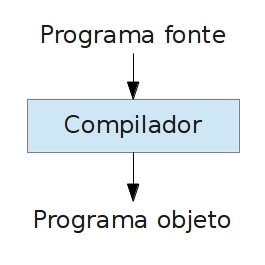
\includegraphics[width=0.25\textwidth]{figuras/compilador}
  \end{center}
  \caption{O funcionamento de um compilador}
  \label{fig:compilador}
\end{figure}

\begin{figure}[htp]
  \begin{center}
    
\includegraphics[width=0.5\textwidth]{figuras/execucao}
  \end{center}
  \caption{Funcionamento de um programa de computador}
  \label{fig:execucao}
\end{figure}

\begin{figure}[htp]
  \begin{center}
    
\includegraphics[width=0.6\textwidth]{figuras/interpretador}
  \end{center}
  \caption{Um interpretador}
  \label{fig:interpretador}
\end{figure}

\begin{figure}[htp]
  \begin{center}
    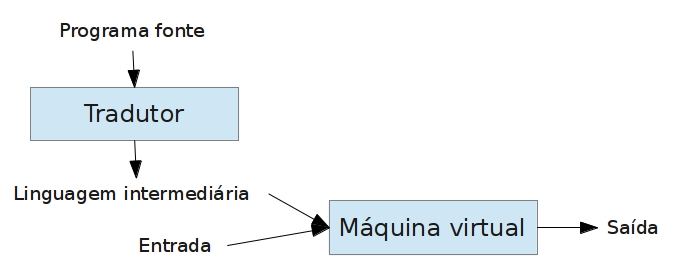
\includegraphics[width=0.6\textwidth]{figuras/hibrido}
  \end{center}
  \caption{Software h\ih brido}
  \label{fig:hibrido}
\end{figure}

\begin{figure}[htp]
  \begin{center}
    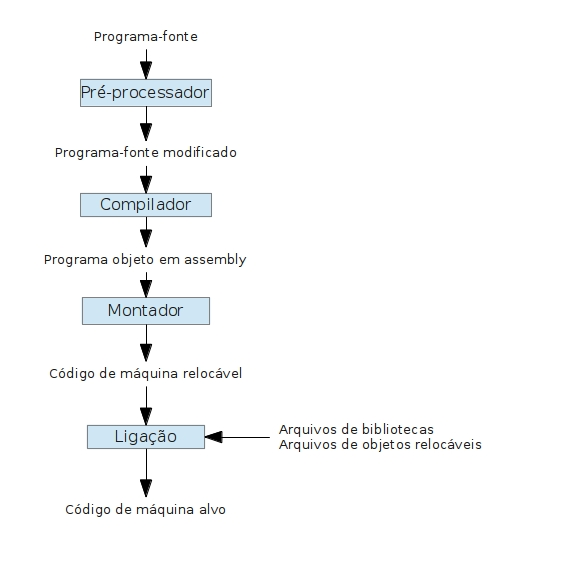
\includegraphics[width=0.7\textwidth]{figuras/gccarch}
  \end{center}
  \caption{GNU Compiler Collection}
  \label{fig:gccarch}
\end{figure}

A figura \ref{fig:gccarch} demonstra a arquitetura do \emph{GCC}\footnote{GNU Compiler Collection}, um dos compiladores mais conhecidos e utilizados para as linguagens C, C++, Objective-C, Fortran, entre outras. Ele \eh\ composto de um \emph{pr\eh -processador}\footnote{\emph{cpp}, que realiza o tratamento das macros de inclus\ao.}, um \emph{compilador}\footnote{\emph{gcc}, para C e \emph{g++} para C++.}, um \emph{montador}\footnote{\emph{as}, que reune os m\oh dulos compilados.} e um \emph{editor de liga\ca o}\footnote{\emph{ld}, que realiza a liga\ca o dos m\oh dulos em tempo de execu\ca o.}.

\emph{M\ah quina Virtual}, segundo \cite{Laureano06} e \cite{IBM11}, \eh\ o software capaz de disponibilizar de forma isolada e  simular o comportamento de uma m\ah quina autom\ah tica ou sistema de processamento de dados, com a capacidade de ampliar a capacidade real da m\ah quina hospedeira.
As m\ah quinas virtuais podem servir a dois objetivos principais:
\begin{description}
\item[Amplia\ca o de hardware] Amplia a capacidade computacional de uma m\ah quina f\ih sica, disponibilizando ao software hospedado, mais mem\oh ria e/ou processadores do que realmente existem;
\item[Homogeneiza\ca o de ambiente de execu\ca o] Padroniza o ambiente de execuc\ca o do programa, muitas vezes permitindo que um mesmo programa possa ser reutilizado em v\ah rias plataformas sem nenhuma ou com poucas altera\co es.
\end{description}

No caso da abordagem h\ih brida, o programa tradutor converte a linguagem \emph{fonte} em uma representa\ca o intermedi\ah ria conhecida como \emph{IL} ou \emph{bytecode}. Esta representa\ca o intermedi\ah ria \eh\ padronizada e permite que o programa interpretador - representado pela m\ah quina virtual leia estes comandos e execute as a\co es apropriadas. H\ah\ tamb\eh m a facilidade de reutiliza\ca o desse programa em representa\ca o intermedi\ah ria entre diferentes plataformas de hardware e sistemas operacionais.

O projeto \emph{LLVM}\footnote{Low Level Virtual Machine.} foi criado para resolver o problema de geração do \emph{melhor código possível}\footnote{O problema de gerar c\oh digo \oh timo \eh\ NP-completo \cite{Aho08}.}, levando em conta as dificuldades geradas pela evolu\ca o das linguagens de programa\ca o e das arquiteturas de computador, permitindo assim maior flexibilidade na cria\ca o, desenvolvimento e estudo de linguagens de programa\ca o.

Na figura \ref{fig:llvmarch} podemos ver a arquitetura de construção do projeto LLVM, consitu\ih da pelo \emph{frontend} (um por linguagem de programa\ca o), respons\ah vel pelo processamento e entendimento da linguagem fonte, de uma especifica\ca o da representação intermedi\ah ria conhecida como \emph{bitcode}\footnote{Originalmente a representa\ca o intermedi\ah ria do LLVM chamava-se \emph{bytecode}, como no Java e no .NET. Com a evolu\ca o do projeto, prestando suporte a um maior n\uh mero de plataformas e arquiteturas, essa especifica\ca o tornou-se bin\ah ria, sendo proposto no f\oh rum do projeto a troca da nomenclatura, por coer\^encia.}, formalmente chamada de \emph{LLVM-IR}\footnote{Low Level Virtual Machine - Intermediate Representation\sigla{LLVM}{Low Level Virtual Machine - Intermediate Representation}.}, seguido pelos passos de otimização (LLVM Optimizer) e finalmente o \emph{backend} (um por arquitetura de hardware) que transforma a representação intermedi\ah ria otimizada em c\oh digo-objeto.

\begin{figure}[htp]
  \begin{center}
    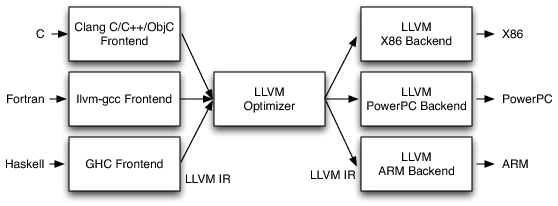
\includegraphics[width=0.7\textwidth]{figuras/llvmarch}
  \end{center}
  \caption{Arquitetura do projeto LLVM}
  \label{fig:llvmarch}
\end{figure}

Na figura \ref{fig:llvmarch2}, vemos mais detalhes de como a arquitetura flex\ih vel do LLVM interage com outros programas e arquivos, realizando a liga\ca o-edi\ca o, otimiza\ca o e otimiza\ca o em tempo de execu\ca o.

\begin{figure}[htp]
  \begin{center}
    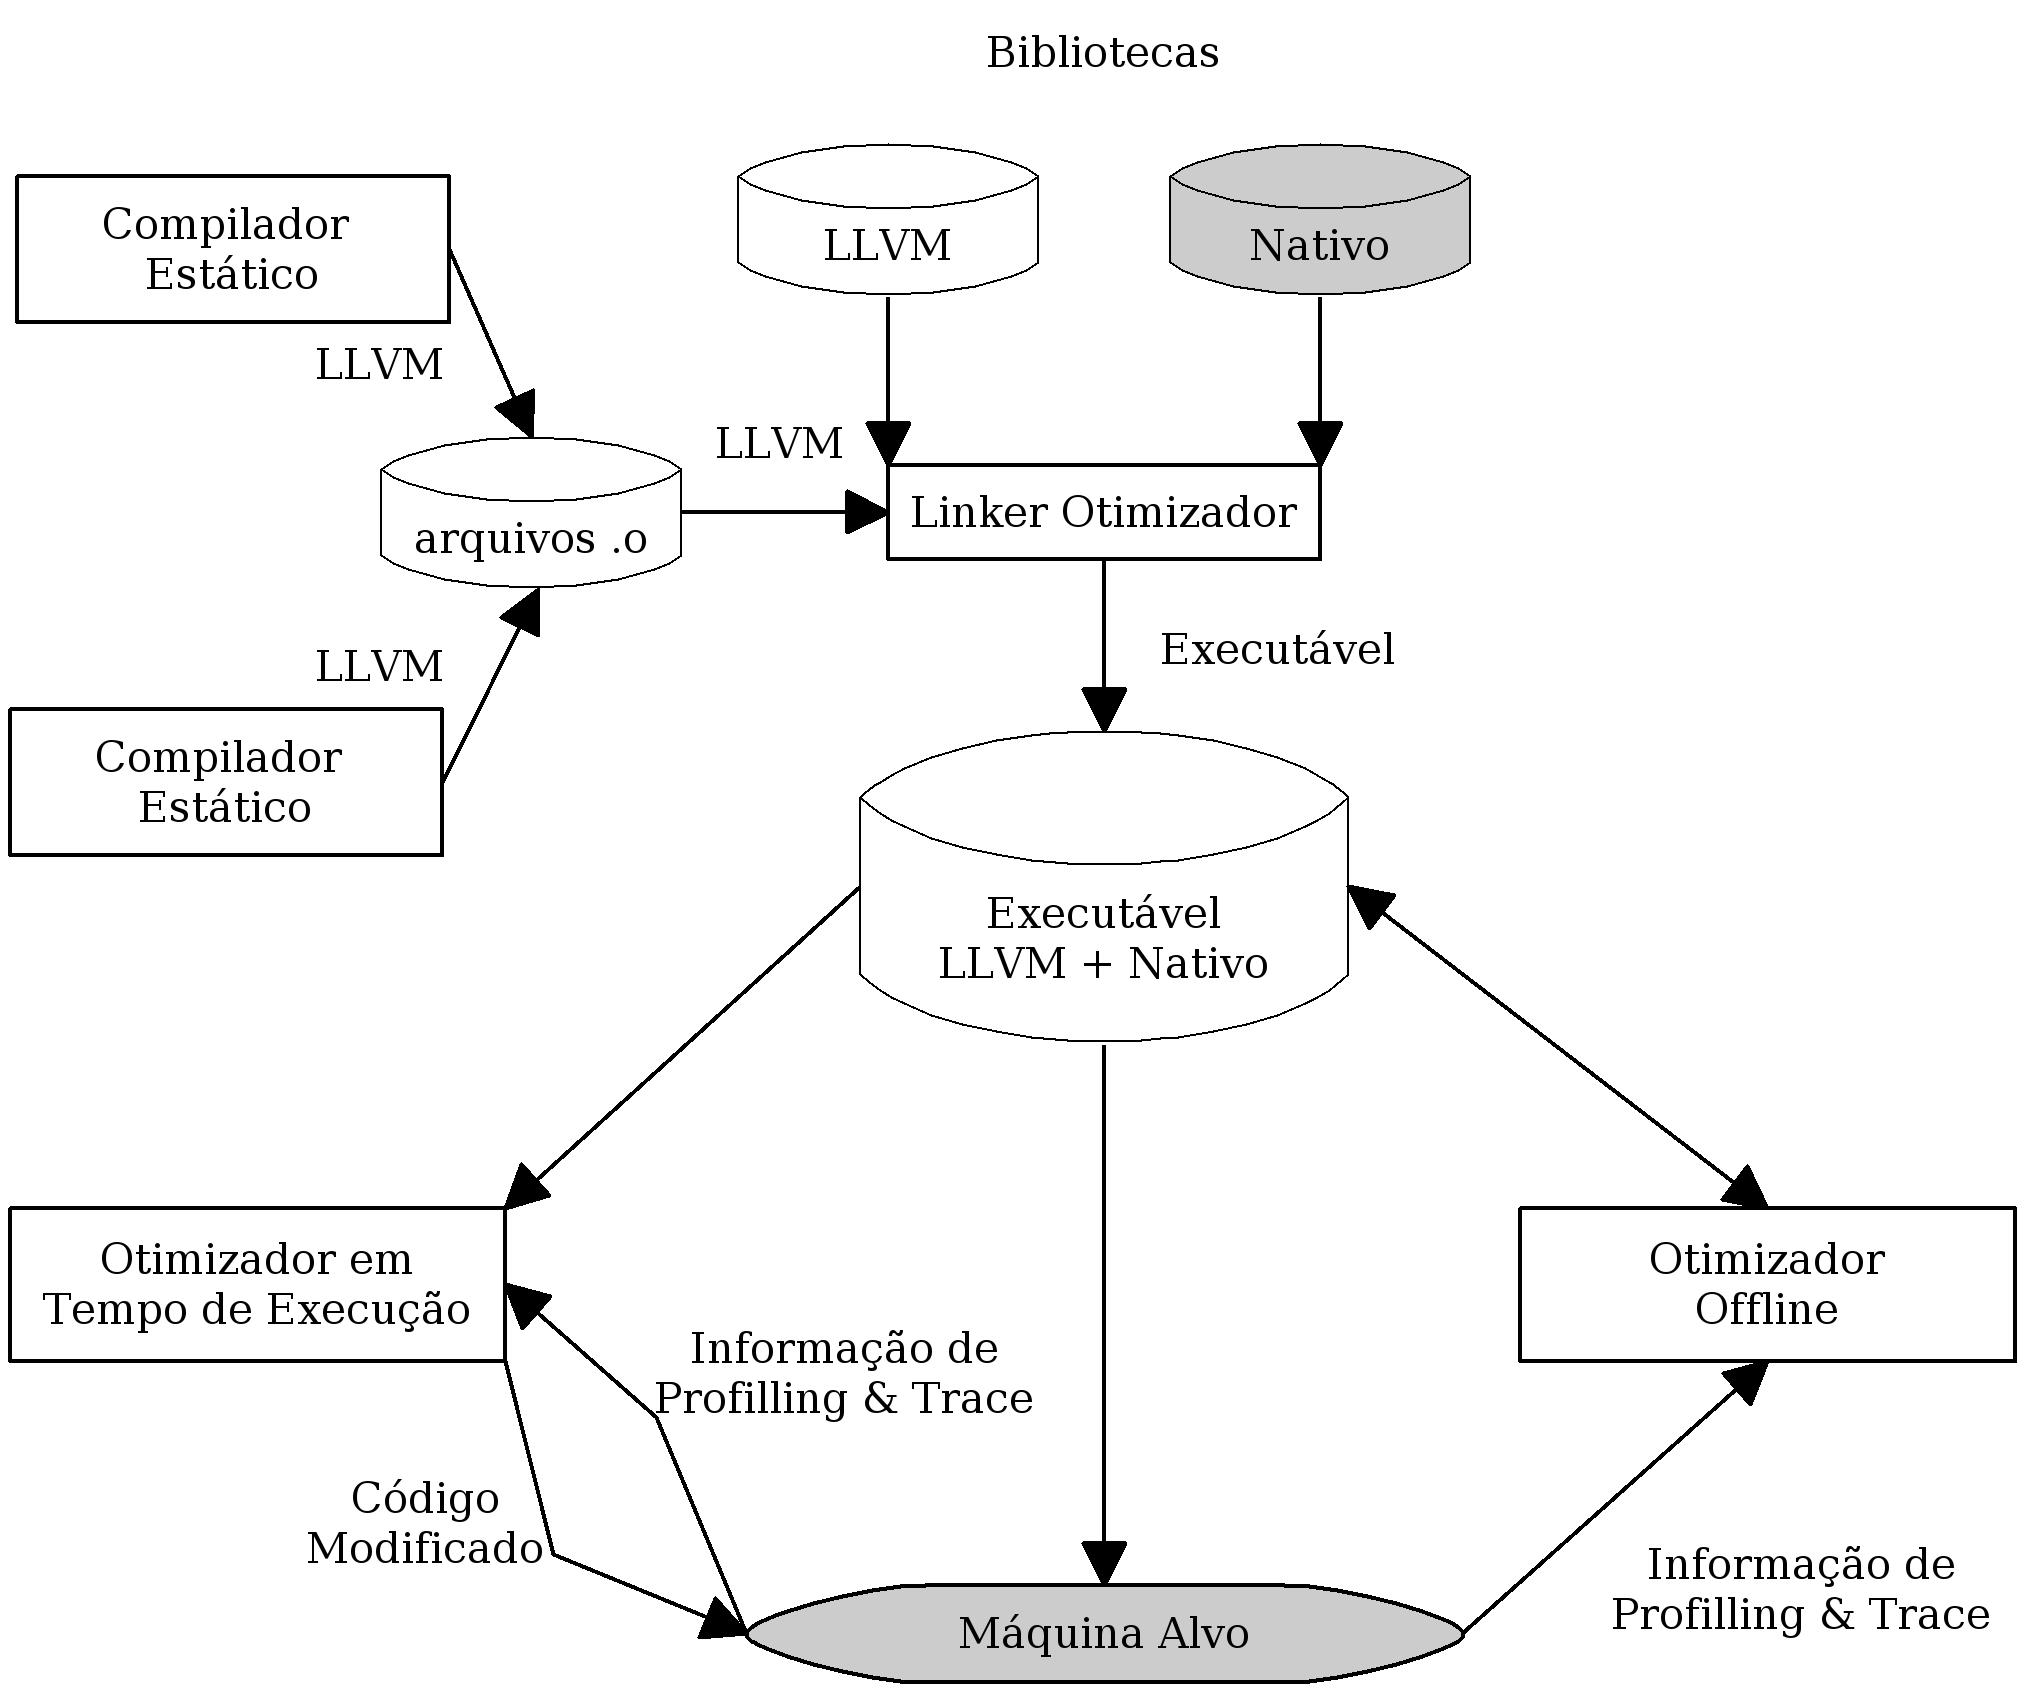
\includegraphics[width=0.7\textwidth]{figuras/llvmarch2}
  \end{center}
  \caption{Arquitetura detalhada do projeto LLVM}
  \label{fig:llvmarch2}
\end{figure}

Segundo \cite{Lattner02},
\begin{citacao}
  LLVM \eh\ desenhado para atingir tr\^es metas:
  \begin{enumerate}
    \item Habilidade de uma estrat\eh gia de otimiza\ca o agressiva em m\uh ltiplos passos, provendo m\ah xima performance;
    \item Servir como um hospedeiro para pesquisa e desenvolvimento, provendo uma funda\ca o forte para projetos atuais e futuros; e
    \item Operar transparentemente para o usu\ah rio final (o desenvolvedor), comportando-se identicamente a um sistema de compilador padr\ao\ (incluindo tempos de compila\ca o realistas).\footnote{N.A. Traduzido pelo autor.}
  \end{enumerate}
\end{citacao}
Levando em considera\ca o que o \emph{frontend} realiza as interpreta\co es da linguagem fonte, o otimizador melhora diversos aspectos da representa\ca o intermedi\ah ria, em v\ah rios n\ih veis de profundidade, seguido pelo compilador JIT e \emph{profiler}\footnote{um \emph{profiler} \eh\ o programa capaz de medir o tempo e n\uh mero de instru\co es utilizadas pelo programa execut\ah vel para realizar determinada tarefa, apontando gargalos de execu\ca o.} embarcado e/ou \emph{offline}\footnote{como o \emph{gprof} que faz parte do GCC, por exemplo.}.

Na cap\ih tulo \ref{pro:descricao}, veremos como o sistema desenvolvido se encaixa na arquitetura do projeto LLVM.

Devido sua arquitetura abrangente e flex\ih vel, o LLVM tem sido utilizado amplamente dentro de institui\co es de ensino para pesquisa e desenvolvimento na \ah rea de computa\ca o, assim como por empresas de tecnologia. Dentre seus utilizadores, podemos destacar: Principled Compilation\footnote{\cite{Carnegie}.}, Cloud9\footnote{\cite{Ecole}.}, Validation of Interprocedual Optimizations\footnote{\cite{NewYork}.}, KLEE\footnote{\cite{Stanford}.}, LENS Framework\footnote{\cite{California}.}, SAFECode\footnote{\cite{Illinois}.}, Hydra Language\footnote{\cite{Adobe1}.}, Alchemy\footnote{\cite{Adobe2}.}, ActionScript 3\footnote{\cite{Adobe3}.}, Xcode\footnote{\cite{Apple1}.}, OS X\footnote{\cite{Apple2}.}, EA\footnote{\cite{EA}.}, Intel\footnote{\cite{Intel}.}, NVIDIA\footnote{\cite{NVIDIA}.}, Siemens\footnote{\cite{Siemens}.}, Sun\footnote{\cite{Sun}.}, iPhone development tools\footnote{\cite{iPhoneDev}.}, Mono\footnote{\cite{Mono}.} e MacRuby\footnote{\cite{MacRuby}.}.

Outro contexto de aplica\ca o do LLVM \eh\ na cria\ca o de interpretadores, j\ah\ que possui um compilador \emph{Just-in-Time}\footnote{\emph{JIT}, permite que o processo de compila\ca o seja embarcado no programa e executado em tempo de execu\ca o.}.

Dentro do contexto de neg\oh cio, h\ah\ cada vez mais uma necessidade por alta performance, confiabilidade e potencializa\ca o dos recursos computacioais das aplica\co es. Poucos ciclos de m\ah quina podem representam, em determinados contextos, a agilidade na realiza\ca o de novos neg\oh cios.

Uma institui\ca o financeira, por exemplo, depende amplamente de otimiza\ca o de seus sistemas, para garantir o maior n\uh mero de transa\co es realizadas no menor tempo poss\ih vel, gerando maiores lucros e clientes mais satisfeitos com sua agilidade e confiabilidade. Ainda neste contexto, vemos uma arquitetura sist\^emica complexa, com diversos sistemas heterog\^eneos, onde predominam linguagens de 2$^{a}$ e 3$^{a}$ gera\ca o como Cobol e C, banco de dados DB2 e Oracle, e plataformas diversas, desde Mainframes at\eh\ celulares\footnote{Tecnologias utilizadas pelos maiores bancos nacionais, como Banco do Brasil e Caixa.}.
